\documentclass[10pt]{extarticle}

\usepackage[english]{babel}
\usepackage{amsmath,amsthm,amssymb,amsfonts}
\usepackage[italicdiff]{physics}
\usepackage[T1]{fontenc}
\usepackage{lmodern}
\usepackage[dvipsnames]{xcolor}
\usepackage[utf8]{inputenc}
\usepackage[paperwidth=5.5cm,paperheight=5.5cm,top=0cm,bottom=0cm,left=0cm,right=0cm]{geometry} %%% Dimensions set to fit cover photo
\usepackage{tikz,tikz-3dplot,tikz-cd,pgf,pgfplots}
\usetikzlibrary{arrows.meta}
\pgfplotsset{compat=newest}

%Created by Senan Sekhon
%Created August 7, 2021

%%% THIS FINE CONTAINS ONLY THE CODE FOR THE PROFILE PICTURE. SEE MAIN FILE FOR THE FULL CODE %%%

\begin{document}

\begin{center}
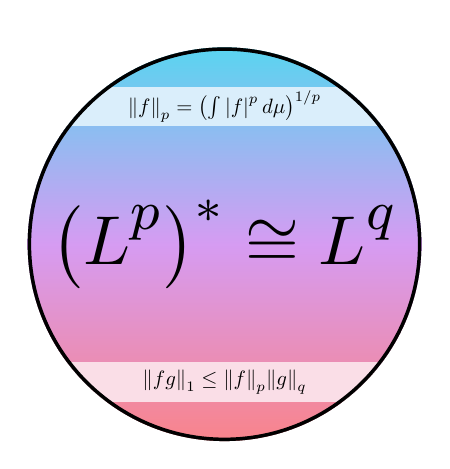
\begin{tikzpicture}[scale=2.5,every node/.style={transform shape}]
\definecolor{tcol}{HTML}{12C2E9} %top color
\definecolor{mcol}{HTML}{C471ED} %middle color
\definecolor{bcol}{HTML}{F64F59} %bottom color

%%% Border for profile picture (to be cropped out)
%\draw (-1.1,-1.1) rectangle (1.1,1.1);
\path (0,1.1)--(0.1,1.1); %this is used to hide the border while ensuring some space above the circular image

%%% Interior and middle text
\fill[very thick,top color=tcol!70,bottom color=bcol!70,middle color=mcol!70] (0,0) circle (1);
\node at (0,0) {$\qty(L^{\raisebox{0.5mm}{\footnotesize\ensuremath p}})^*\cong L^{\raisebox{0.5mm}{\footnotesize\ensuremath q}}$};

%%% Stripes and text within stripes
\clip (0,0) circle (1); %crop for stripes
\fill[bcol!70!mcol!20] (-1,-0.8) rectangle (1,-0.6);
\fill[tcol!70!mcol!20] (-1,0.6) rectangle (1,0.8);
\node[scale=0.3] at (0,0.7) {$\norm{f}_p=\qty(\int\abs{f}^p\,d\mu)^{1/p}$};
\node[scale=0.3] at (0,-0.7) {$\norm{fg}_1\le\norm{f}_p\norm{g}_q$};

%%% Circle outline
\draw[line width=2.5pt] (0,0) circle (1);
\end{tikzpicture}
\end{center}

\end{document}